\documentclass[10pt,a4paper]{article}
\usepackage[utf8]{inputenc}
\usepackage{amsmath}
\usepackage{amsfonts}
\usepackage{amssymb}
\usepackage{graphicx}
\usepackage{verbatim}
\usepackage{float}
\usepackage{tikz}
\usepackage{subfig}
\usepackage{tcolorbox}
\usepackage{parskip}
\usepackage[left=2cm,right=2cm,top=2cm,bottom=2cm]{geometry}
\author{Songtuan Lin u6162630}
\title{Computer Network}
\begin{document}
\maketitle

\section{Basic Terminology}
Network, particularly in terms of Computer Science, is consist of several devices that are able to \textit{communicate} with each other. The term \textit{communicate} here means the device within Network can send or receive message from other devices. In order to perform this communication, each device within Network must be able to be located, or simply speaking, each device must have a \textit{address}. There are several methods to assign \textit{addresses} to devices, each of them corresponding to a specific technology that is used to construct Network. One popular technology is \textit{Internet}, which assign a \textit{IP} to each device within Network as their address. In here, \textit{Internet} is the technology that used to construct Network and \textit{IP} is the method that Internet used to address(locate) devices within it. 

Furthermore, in order to let devices within Network communicate with each other, one essential requirement is that there must be a thing that can carry the message and deliver it between devices. Such thing, which can be called as \textit{media}, consist the \textit{Physical Layer} of Computer Network

\section{Physical Layer}
As described in last section, \textit{Physical Layer} is consist of the media that can carry and deliver messages. Particularly, as Figure \ref{physical_layer} illustrated, the media is the line that connect Device A and B. 
\begin{figure}[ht]
	\center
	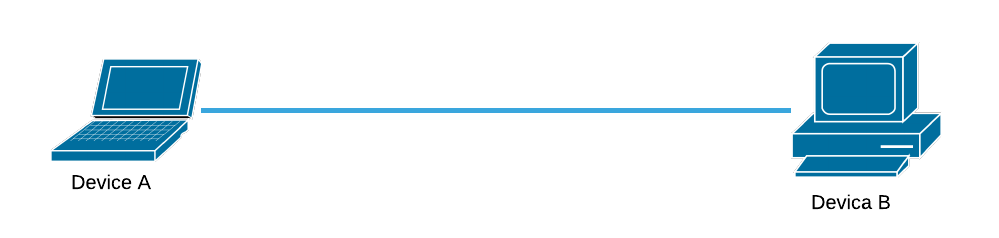
\includegraphics[scale=0.85]{Physical}
	\caption{Media between Different Devices}
	\label{physical_layer}
\end{figure}
Furthermore, based on the characteristics of the media, it can be categorized into following three classes::
\begin{enumerate}
	\item \textbf{Simplex}: This type of media can only transport message with a \textit{fixed direction}, \textsl{e.g.} from Device A to Device B.
	\item \textbf{Half-Duplex}: This type of media can transport message with both directions. However, it can only choose one direction during each transportation, \textsl{e.g.} from A to B or B to A.
	\item \textbf{Duplex}: This type of media can transport message with both direction during a transportation, \textsl{e.g.} transport message from A to B and B to A in the same time.
\end{enumerate}
Indeed, the Figure \ref{physical_layer} give us an inspiration about how to construct a simple network, which is connecting each devices within network with a media. For example. assume we want to construct a Network contain four devices, the easiest way to do this is shown in Figure \ref{topology_basic}, in which, each device is connected with the rest.
\begin{figure}[ht]
	\center
	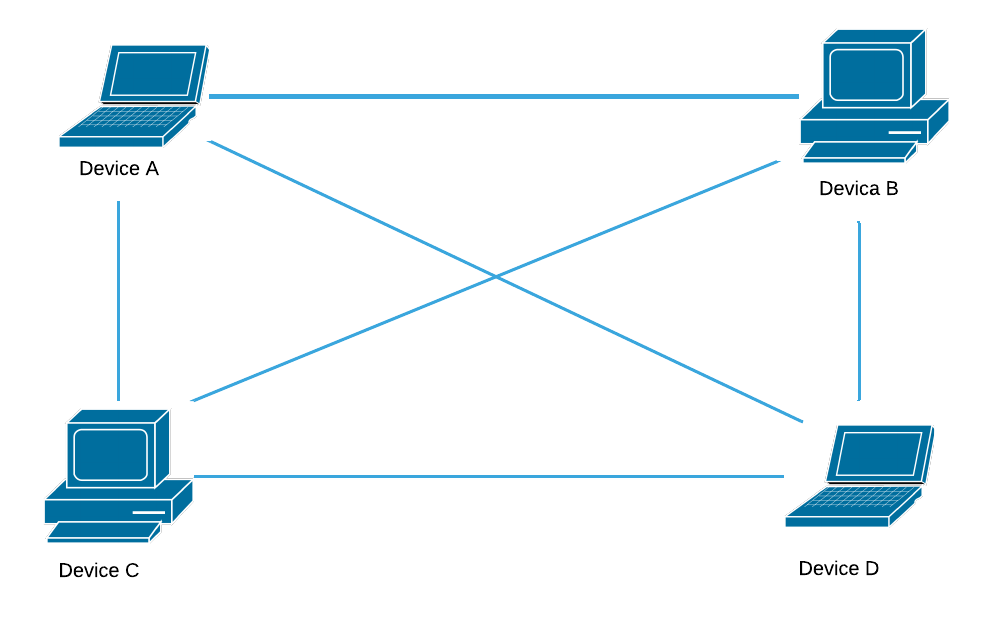
\includegraphics[scale=0.5]{Topology}
	\caption{Basic Topology}
	\label{topology_basic}
\end{figure}
However, the problem of this topology is that the number of medias will grow exponentially with the increasing number of devices. Therefore, an improvement topology along with an algorithm(protocol) to control how the messages are delivered is required, which relate to our next topic: \textit{Data-Link Layer}

\section{Data-Link Layer}
The solution of the problem remaining in last section is straightforward: By adding one or more \textit{Switch} which depend on the number of devices within network. The Switches work as bridges that connect different devices in Network, as illustrated in Figure \ref{topo}:
\begin{figure}[ht]
\center
\subfloat[]{\begin{tikzpicture}
	\node[label=below:Device] (laptop_1) at (6, 3){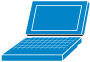
\includegraphics[scale = 0.3]{laptop}};
	\node[label=below:Switch] (switch) at (3, 3){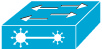
\includegraphics[scale = 0.3]{switch}};
	\node[label=below:Device] (laptop_2) at (0, 3){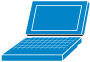
\includegraphics[scale = 0.3]{laptop}};
	\node[label=right:Device] (laptop_3) at (3, 1){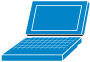
\includegraphics[scale = 0.3]{laptop}};
	\node[label=right:Device] (laptop_4) at (3, 5){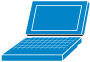
\includegraphics[scale = 0.3]{laptop}};
	
	\draw[blue, thick] (laptop_1) -- (switch);
	\draw[blue, thick] (laptop_2) -- (switch);
	\draw[blue, thick] (switch) -- (laptop_3);
	\draw[blue, thick] (switch) -- (laptop_4);
\end{tikzpicture} \label{topo_1}} \\

\subfloat[]
{
	\begin{tikzpicture}
		\node[label=below:Device A] (laptop_1) at (1, 4){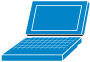
\includegraphics[scale=0.3]{laptop}};
		\node[label=below:Device B] (laptop_2) at (1, 2){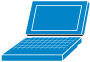
\includegraphics[scale=0.3]{laptop}};
		\node[label=below:Switch A] (switch_1) at (3, 3){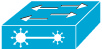
\includegraphics[scale=0.3]{switch}};
		\node[label=below:Switch B] (switch_2) at (5, 3){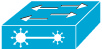
\includegraphics[scale=0.3]{switch}};
		\node[label=below:Device C] (laptop_3) at (7, 4){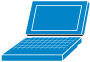
\includegraphics[scale=0.3]{laptop}};
		\node[label=below:Device D] (laptop_4) at (7, 2){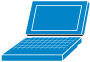
\includegraphics[scale=0.3]{laptop}};
		
		\draw[blue, thick] (laptop_1) -- (switch_1);
		\draw[blue, thick] (laptop_2) -- (switch_1);
		\draw[blue, thick] (switch_1) -- (switch_2);
		\draw[blue, thick] (switch_2) -- (laptop_3);
		\draw[blue, thick] (switch_2) -- (laptop_4);
	\end{tikzpicture}
	\label{topo_2}
}
\caption{Two Example of Network Topology}
\label{topo}
\end{figure}
Even though the switches reduce the number of connection, the new problem is how the the different devices communicate with each other under the condition that they are not direct connected. This problem may be better illustrated by an example: Assume Device A in Figure \ref{topo_2} is willing to send a message to Device D. The first thing Device A need to do is locating Device D, or we can say, Device A need to find the \textit{address} of Device D. The address here is called \textit{MAC address} and in order to find Device B's MAC address, Device A will \textit{broadcast} a request message which contain a query: "What is the MAC address of Device B" and it's own MAC address. The \textit{broadcast} here means A will send this query to all the devices within this Network(Device B, C and D). In order to indicate this query is a broadcasting message, Device A will set the destination MAC address of this query as a special value: FF-FF-FF-FF-FF-FF and send it to Switch A. When Switch A receives this query and recognizes this message is a broadcasting message as it has FF-FF-FF-FF-FF-FF as destination MAC address, Switch A will send this query to every device it connect to, include both Device B and Switch B. Furthermore, when Switch A receive this query, it will record the source MAC address of this query(Device A's MAC address) along with the index of port that receive this query into a table, \textsl{e,g} Switch A will record the pair:
\begin{center}
	\begin{tabular}{|c|c|}
		\hline
		Device A's MAC address & Port 5 \\
		\hline
	\end{tabular}
\end{center}
into the table if the query message come through port 5 of Switch A. This table is called \textit{ARP table}. By maintain such a table, when Switch A receive a message which has Device A's MAC address as destination, it can directly forward this message to Device A through port 5 by searching Device A's MAC address along with the corresponding port within ARP table. After Switch A broadcast the query, Switch B and Device B will both receive this query message. Device B will realize that Device A did not ask its' MAC address and will simply discard this query message without further action. By contrast, Switch B will keep this broadcasting which finally cause Device D receive this query. One thing that need to be noticed is that Switch B will also record Device A's MAC address and the corresponding port index into ARP table by reading the source MAC address within query message. When Device D receive this query, it will response Device A with a respond message which use Device A's MAC address as destination address, its' own MAC address as source address and carry its' MAC address as query result. This respond message will be transferred back to Device A through Switched with the Device D's MAC address(source address) be recorded into each Switch's ARP table. After Device A receive the MAC address of Device D, it can then send the further message by setting Device D's MAC address as destination address. The Switch can also know which port should be used to send these messages by searching the ARP table to find Device D's MAC address. 

It can be seen from the above procedure, in order to perform message delivering within this Network topology. The messages must have some specific content, \textsl{e.g.} source address and destination address, or without loss generality, we can say, the messages that being transferred under this mechanism must have s specific format. This message delivering mechanism with specific message format is called \textit{protocol} and the message delivering mechanism within the Network topology described above is called \textit{ARP Protocol}. 

Indeed, we can give the messages that flowing within this Network a name: \textit{Ethernet Frame}. According to above discussion, we know that Ethernet Frame must follow a specific format. The exact Ethernet Frame format is:
\begin{center}
	\begin{tabular}{|c|c|c|c|c|c|}
		\hline
		Preamble & Destination Address & Source Address & Type & Actual Message Content & CRC code \\
		\hline
	\end{tabular}
\end{center}
In which, the most two important field: Destination Address and Source Address, have been introduced in the previous part.

\subsection{Wireless Connection}

The most content we discussed in these two sections is based on the wired connection, or we can say, use physical line as media in Physical Layer. However, in recent years, the wireless connection become more and more popular. By using wireless connection, one device can communicate with the other without using physical line. Indeed, this wireless connection technology is not as fancy as many people think. In wireless network, the devices use wireless connection connect to a \textit{base station} and this base station will connect to the normal wired network topology as described before. So, an example wireless network is:
\begin{figure}[ht]
	\center
	\begin{tikzpicture}
		\node[label=right: Device A] (laptop_A) at (-2, 2){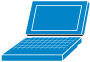
\includegraphics[scale=0.3]{laptop}};
		\node[label=right: Device B] (laptop_B) at (-2, -2){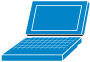
\includegraphics[scale=0.3]{laptop}};
		\node[label=below: Base Station] (base_station) at (0, 0){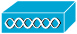
\includegraphics[scale=0.3]{accesspoint}};
		\node[label=below: Switch] (switch) at (2, 0){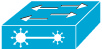
\includegraphics[scale=0.3]{switch}};
		\node[label=center: Network Topology as Figure \ref{topo_2}] (cloud) at (6, 0){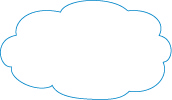
\includegraphics[scale=0.9]{cloud}};
		
		\draw[blue, dashed, thick] (laptop_A) -- (base_station);
		\draw[blue, dashed, thick] (laptop_B) -- (base_station);
		\draw[blue, thick] (base_station) -- (switch);
		\draw[blue, thick] (switch) -- (cloud);
	\end{tikzpicture}
	\caption{Wireless Network Topology}
	\label{wireless}
\end{figure}
In which, the dashed line between Device A, B and Base Station denote the wireless connection. The name of base station and the function it provide may varied depend on what wireless communication protocol it is used. Particularly, in \textit{802.11 protocol}, which is the protocol we will focus on, the base station is given name: \textit{access point} or \textit{AP}. Furthermore, since wireless connection is more unstable than wired connection, the majority wireless protocols, include 802.11, require message receiver to send a acknowledgment back to message sender so that the sender can know this message has been successfully received. Before we move to more detail of 802.11 protocol, there is one more problem that we need to realized: In Figure \ref{wireless}, even though we only draw the wireless connection between Devices and Base Station, the message sent or received by one device will indeed being received by all the others, which means, the message sent by one device will be broadcast to all the other device that connect to the same base station. Hence, the equivalent topology of wireless connection can be illustrated as Figure \ref{equivalent}, which indicated these devices are actually sharing a communication line.
\begin{figure}[ht]
	\center
	\begin{tikzpicture}
		\node[label=right: Device A] (laptop_A) at (0, 2){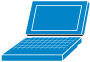
\includegraphics[scale=0.3]{laptop}};
		\node[label=below: Device B] (laptop_B) at (2, -2){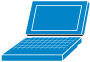
\includegraphics[scale=0.3]{laptop}};
		\node[label=below: Base Station] (base_station) at (5, 0){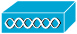
\includegraphics[scale=0.3]{accesspoint}};
		\draw[blue, thick] (-1, 0) -- (base_station);
		\draw[blue, thick] (laptop_A) -- (0, 0);
		\draw[blue, thick] (laptop_B) -- (2, 0);
	\end{tikzpicture}
	\caption{Equivalent Wireless Connection}
	\label{equivalent}
\end{figure}
The problem of this connection is straightforward: When there are more than one device are sending messages through this line, these messages will have collision with each other, and hence cause the messages be corrupted. The solution of this problem is a protocol called \textit{CSMA/CA} stand for \textit{Carrier Sense Multiple Access with Collision Avoid}. The CSMA/CA protocol work as follow: When a device have a message to be sent, it will:
\begin{enumerate}
	\item Check whether the line is idle(no message is currently transferring on it). If the line is idle, the device will start to transfer message after a fixed small period of time known as \textit{Distributed Inter-frame Space}(DIFS).
	\item If the line is not idle, the device will choose a random delay time and set up a timer to count down this value. One thing that need to be noticed here is the timer only start to count down when the device senses the line is idle, which means, the timer will freeze if there are messages being transferred through the line. 
	\item When the timer count down to zero, the device will start to transfer the message and wait to receive the acknowledgement.
	\item If the acknowledgement is received, the device know this message has been received. Otherwise, device will go back to step 2 and choose a delay time to prepare to re-transmit this message.
\end{enumerate} 
The reason for using DIFS is that: There will always be a transmission delay between Device A and Device B which caused by the distance between A and B. Hence, when Device A start to transfer a message, Device B will sense the line is idle until the message reach the location of B. Hence, if B start to transfer message at this time period(the time that the message hasn't reach B but the line is actually not idle), the collision will happen. The DIFS is designed to try to avoid this time period and hence, further decrease the probability that collision happen.

After we have described some fundamental mechanism of wireless connection, we can now start to discuss some detail about 802.11 protocol. The most important question is: How the device connect to AP(base station). In order to connect to a AP, the first thing a device need to do is to figure out which AP it will connect to, or in more generally, device need to know the identification of each AP so that it can choose which one to connect to. In 802.11, each AP is identified by a \textit{Service Set Identifier}(SSID) and will be used by device as its' identification. Even though the SSID provide a method that allow device to know the identification of each AP, device still need to know the list of APs(identified by SSID) that it can connect to and then establish the connection, 802.11 provide two mechanisms to achieve this goal:
\begin{description}
	\item[Passive Scanning]: The procedure of passive scanning is:
	\begin{enumerate}
		\item Each AP will broadcast a \textit{Beacon Frame} which inform the devices within this area with its' SSID and told them it is willing to be connected.
		\item Each device will receive multiple Beacon Frame and hence get a list of APs it can connect to. The device will select one of them and send a \textit{Request Frame} to request establishing a connection with this AP.
		\item The chosen AP will respond with a \textit{Response Frame} to confirm the connection is established.
	\end{enumerate}
	\item[Active Scanning]: The procedure of active scanning is:
	\begin{enumerate}
		\item Each device will broadcast a \textit{Prob Request Frame} to each AP to request APs' SSID.
		\item When AP receive this Prob Request Frame, it will respond with a \textit{Probe Response Frame} which indicate its' SSID.
		\item The device will get a list of available APs by receiving multiple Probe Response Frame. The device will choose one AP and send a Request Frame to request establishing connection.
		\item The chosen AP will respond with a Response Frame to confirm the connection is established.
	\end{enumerate}
\end{description}

\section{Network Layer}
The Network Topology described in above section is usually called \textit{Local Area Network}(LAN). LAN is actually a successful Network that can allow different devices communicate with other. However, the problem raise with the increasing number of devices, especially when some part of devices may have very long distance with the others. The topology of LAN is definitely not suitable for this large scale Network for the reasons:
\begin{enumerate}
	\item The large number of Switched are required so that them can connect all the devices, which will cause the Network Topology become missive and raise a lot of problems such as \textit{Broadcasting Storm}.
	\item The large of number of long wire is required to connect the devices that cross long distance, which increases the cost significantly. 
\end{enumerate}
In order to address these problem, we first consider that the function provided by Data-Link Layer already guarantees the messages can be successfully delivered within LAN. Therefore, we can separate this big massive Network into different LANs and build a new mechanism that can deliver message from one LAN to the other, which means, we can build a new Layer that control how message will be transferred from one LAN to the other upon he original Data-Link Layer by using the functions(services) provided by Data-Link Layer. In more generally, what we are doing is think each LAN as a single device and build a mechanism to transfer message between them, as illustrated in Figure \ref{network_layer}.
\begin{figure}[ht]
	\center
	\begin{tikzpicture}
		\node[label=center: LAN 1] (LAN_1) at (-4, 2){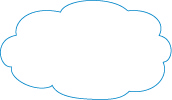
\includegraphics[scale=0.3]{cloud}};
		\node[label=center: LAN 2] (LAN_2) at (-4, -2){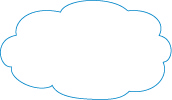
\includegraphics[scale=0.3]{cloud}};
		\node[label=left: Router 1] (router_1) at (-2, 0){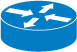
\includegraphics[scale=0.3]{router}};
		\node[label=below: Router 2] (router_2) at (2, 0){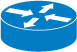
\includegraphics[scale=0.3]{router}};
		\node[label=right: Router 3] (router_3) at (0, 2){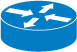
\includegraphics[scale=0.3]{router}};
		\node[label=center: LAN 3] (LAN_3) at (0, 4){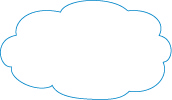
\includegraphics[scale=0.3]{cloud}};
		\node[label=center: LAN 4] (LAN_4) at (5, 0){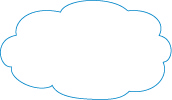
\includegraphics[scale=0.3]{cloud}};
		
		\draw[blue, thick] (LAN_1) -- (router_1);
		\draw[blue, thick] (LAN_2) -- (router_1);
		\draw[blue, thick] (router_1) -- (router_2);
		\draw[blue, thick] (router_3) -- (LAN_3);
		\draw[blue, thick] (router_2) -- (router_3);
		\draw[blue, thick] (router_1) -- (router_3);
		\draw[blue, thick] (router_2) -- (LAN_4);
	\end{tikzpicture}
	\caption{Illustration of Network Layer Topology}
	\label{network_layer}
\end{figure}
As what we have done in LAN, we still need a device to connect each LAN. This device, in term of Network Layer, is called \textit{Router}. The Router which directly to a LAN is called this LANs' \textit{Gateway Router} as this Router is the gate that allow this LAN to communicate with the other LANs. As usual, the first thing to do to build a successful message delivering mechanism is to locate each LAN, or generally speaking, to find the address of each LAN. This bring us the concept of \textit{IP address} and \textit{Sub-net Mask}.

\subsection{IP Address and Sub-net Mask}
IP address is the address of device in term of Network Layer. IP address is coded under base 2 and using 32 bits, \textsl{e.g.}:
\begin{equation*}
	x_{1} x_{2} x_{3} \cdots x_{32}
\end{equation*}
Where each $x_{i} \in \{ 0, 1 \}$. Usually, the IP address is divided into 4 group each contain 8 bits:
\begin{equation*}
	x_{1} x_{2} \cdots x_{8} \quad x_{9} x_{10} \cdots x_{16} \quad x_{17} x_{18} \cdots x_{24} \quad x_{25} x_{26} \cdots x_{32}
\end{equation*}
And transfer each 8-bit binary number to 10-base number, we then get out familiar format IP address: $x.x.x.x$. Particularly, when we assign IP address to device, the devices within the same LAN \textit{must} have the same prefix. \textsl{e.g.} the first 24 bits of IP addresses for each device within LAN 1 must be the same. A example may help better illustrate this idea: If the IP address for device A in this LAN is 192.168.1.1, then, the IP address for device B must be something like $192.168.1.x$ where $1 < x < 255$ as the first 24 bits, corresponding to $192.168.1$, must be the same for all devices within this LAN. Indeed, we usually use \textit{Sub-net Mask} to indicate the length of prefix for each LAN. The sub-net mask is also a 32-bit binary number, if a LAN has a $x$-bit prefix, then, the first $x$ bits of its' sub-net mask will be set to 1 and the rest $32-x$ bits will be set to zero. For example, a LAN has a prefix length equal to 20 bits, then, its' sub-net mask is:
\begin{equation*}
	\underbrace{111 \cdots 11}_{20 \, bits}\underbrace{000 \cdots 00}_{12 \, bits}
\end{equation*}
We can also divide the 32-bit sub-net mask into 4 groups each contain 8 bits and then, turn each group into 10-base number, \textsl{e.g.} a sub-net mask that indicate 24-bit length prefix can be written as $255.255.255.0$ under this transformation.

Indeed, by combining the devices' IP address along with the prefix-length of the LAN this device belong to, we have the form $x.x.x.x/y$, the term $x.x.x.x$ indicate the device's IP address and $y$ indicate the prefix length. We notice that the form $x.x.x.x/y$ not only specific the devices' IP address, but indicate which LAN it belong to. By inspiration of this, we notice that each LAN can be identified by its' prefix. For example, for a LAN, the device within this LAN has the IP address $192.168.1.x/24$, which means, for each device within this LAN, the first 24 bits of their IP address, which is $192.168.1$ must be the same. On the other word, the prefix of this LAN is $192.168.1$. therefore, we can use this first 24 bits prefix as the address of LAN and set the rest bits to zero. As a result, the address of this LAN is $192.168.1.0/24$. The term $/24$ cannot be omitted as it may cause some mistakes in some cases. For example $192.168.1.128/25$ denote the address for a LAN as the first 25 bits is the prefix. However, it can become a legal IP address within a LAN $192.168.1.0/24$.

\subsection{Message Delivering}
After we have identified the address of LAN, we can start to build the mechanism for message delivering. Since the topology of Network Layer is far more complicated than LAN topology (it usually has a lot of Routers), the mechanism similar to ARP protocol can not be used in here. Instead, in Network Protocol, we explicitly calculate the route for message delivering. The protocols that target for this task include OSPF, RIP, etc.

\subsection{Revision of Message Delivering within LAN}
Recall the ARP protocol used in Data-Link Layer. In the beginning, the message sender A will send a ARP request that ask: What is the MAC Address of B. In here, B is actually identified by its' IP address, let's assume B's IP is 192.168.1.10/24, then, what ARP Request message actually ask is: What is the MAC Address of 192.168.1.10/24. After A get the ARP Response, A will record the B's IP along with it's MAC address into a ARP table. Then, when A want to send some further message, it can get B's MAC address directly from the ARP table.

The above situation happened when A, B are in the same LAN, what if A, B are in different LAN? In the beginning, A will notice B is in a different LAN as their prefix is different. Hence, A will deliver this message to B's LAN through Network Layer. When this message reach LAN B's Gateway Router, this router will deliver the message to B through Data-Link Layer, which means, bu using ARP protocol.






















\begin{comment}
Therefore, one improvement is by adding an extra device that connect with the original four devices, as shown in Figure \ref{topology_2}.The added device connect with the rest four devices, hence, these four devices can communicate with each other through this central device.
\begin{figure}[ht]
	\center
	\subfloat[]{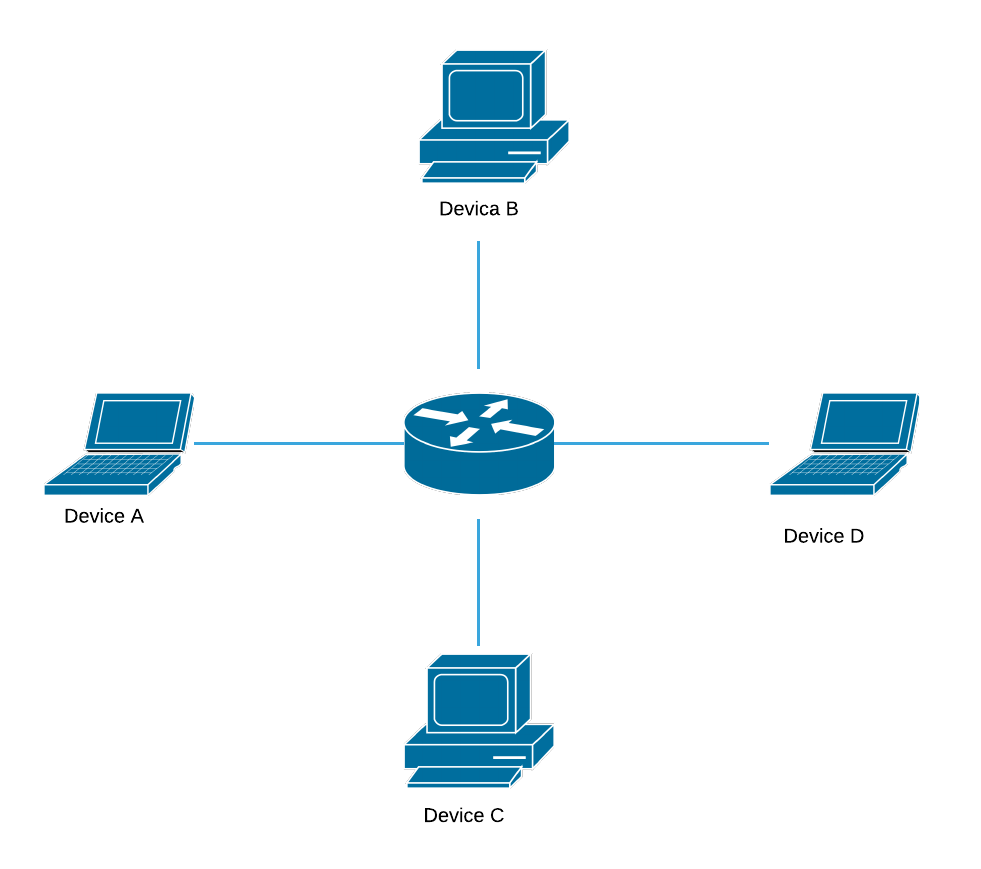
\includegraphics[scale=0.35]{Topology_2} \label{topology_2}}
	\hspace{1cm}
	\subfloat[]{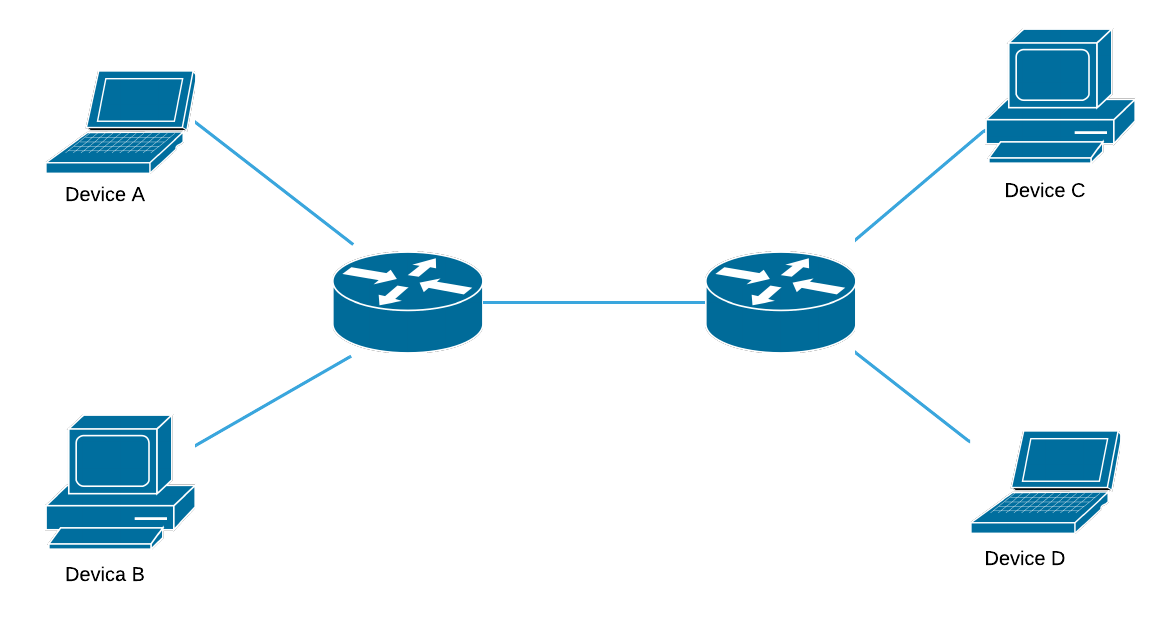
\includegraphics[scale=0.35]{Topology_3} \label{topology_3}}
	\caption{Improvement Topology}
	\label{topology_improvement}
\end{figure}
However, this topology also has the following drawbacks:
\begin{enumerate}
	\item The central device is easy to be overload if there are too many devices connect to it.
	\item It will cost a lot if there are several devices located far away from this central device, \textsl{e.g.} if device C and D is far away from central device, then, the cost to link central device with C and D will be pretty high.
\end{enumerate}
The solution for these two problems is straightforward: By adding more extra devices, as illustrated in Figure \ref{topology_3}. In which, we can assume that device A(C) and B(D) locate in the same area and have relative short distance. Particularly, we can assume device A and B are the computers in one building and device C and D are computers in the other, therefore, we can first connect A, B with one added device and C, D with the other. After that, we can connect these two added devices with each other and hence connect the whole network. Compare with the topology in Figure \ref{topology_2}, this topology has the advantages:
\begin{enumerate}
	\item Is much cheaper as there is only one long-distance connection which happen between the two added devices.
	\item Is much stable as the two added devices do not need to take too much workload compare with the central device in Figure \ref{topology_2}.
\end{enumerate}
Particularly, these added devices, in both Figure \ref{topology_2} and \ref{topology_3}, are called Router and will be explained in further sections. Additionally, the single message that is delivered is called package in terms of Computer Network. 

By the end of this section, we can conclude that the media in Physical Layer is responsible for transferring the message by using its' physical property. However, we still need to define some further mechanisms that control how the message will be delivered, which is the purpose of \textit{Data-Link Layer}. Before we go into these detail, we will first introduce some more high-level thing relate to Computer Network.

Even though the connection between two devices within Network may be complicate, \textsl{e.g.} went through many middle devices like Figure \ref{topology_3}, we can abstract this complicate connection as a direct link that connect the two device and handle the message transportation task, as shown in Figure \ref{virtual}:
\begin{figure}[ht]
	\center
	\subfloat[Real Connection between Two Devices]{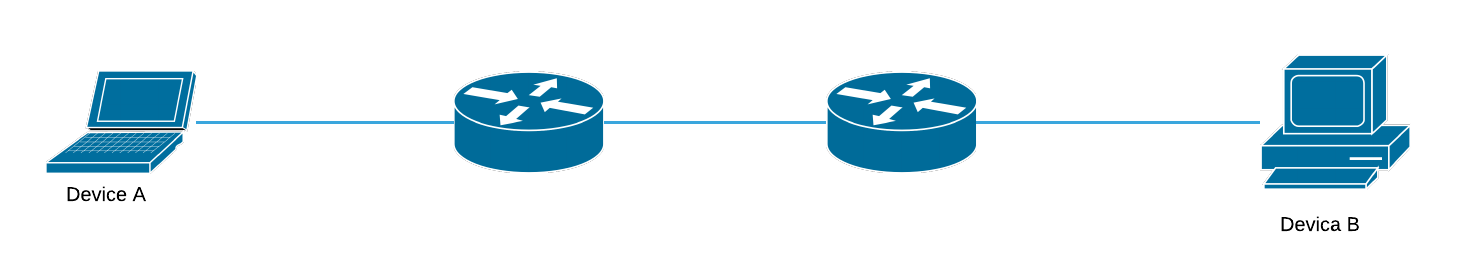
\includegraphics[width = 0.5\textwidth]{Real_Link}  \label{real_link}}
	\vspace{1cm}
	\subfloat[Virtual Connection between Two Devices]{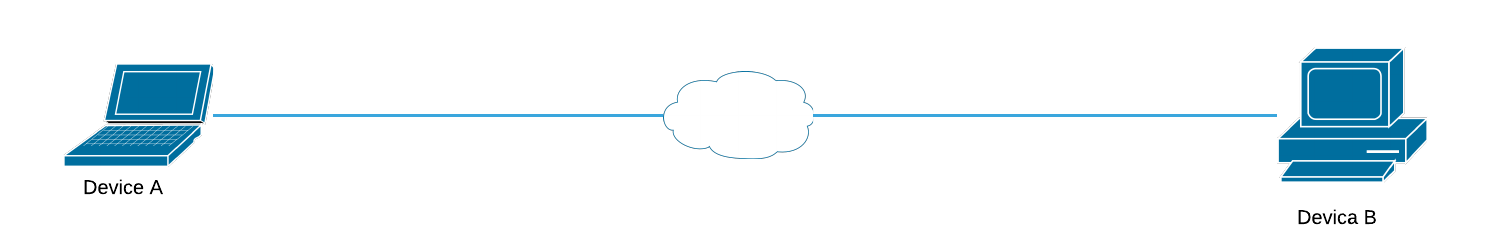
\includegraphics[width=0.55\textwidth] {Virtual_Link} \label{virtual_link}}
	\caption{Virtual Link}
	\label{virtual}
\end{figure}
Figure \ref{real_link} show the real connection between device A and B, which contain two Routers. Figure \ref{virtual_link} abstract this connection as a virtual link. Therefore, from device A and B's perspective, they are directly connecting with each other. Indeed, this virtual link, or we can say, the transportation service provided by the real connection, has the following characteristics to measure it performance:
\begin{enumerate}
	\item \textbf{Reliable}: Measure the frequency of the error that happened during the transmission.
	\item \textbf{Throughput}: Measure the maximum number of packages that can be delivered through this link per second.
	\item \textbf{Delay}: Measure the time that one package transported from one device to the other should take.
\end{enumerate}
This concept of virtual link allow the application within devices do not need to worry about the message transmission, instead, the application can focus on the generation and processing of messages. 
Indeed, one kind of communication that usually happen within Network is that: One device request a file that store in other device. In this case, the device that send the request is called \textit{client} and the device that store the file is called \textit{server}. The communication process is straightforward: The client first send the request to server and the server response with the corresponding file. However, for some servers, it may need to process huge number of request, which will easily cause the server overload. Therefore, an improvement architectural of server is required to handle this problem.

\section{3-Tier Server Architectural}
As mentioned in last part, some server may need to process a lot messages. Therefore, one single device is not enough under this situation as single device do not have ability to handle so much request. One solution is by adding more devices and separate the server into 3 part, in which, each part is corresponding to a specific task, as illustrated in Figure \ref{server}:
\begin{figure}[ht]
	\center
	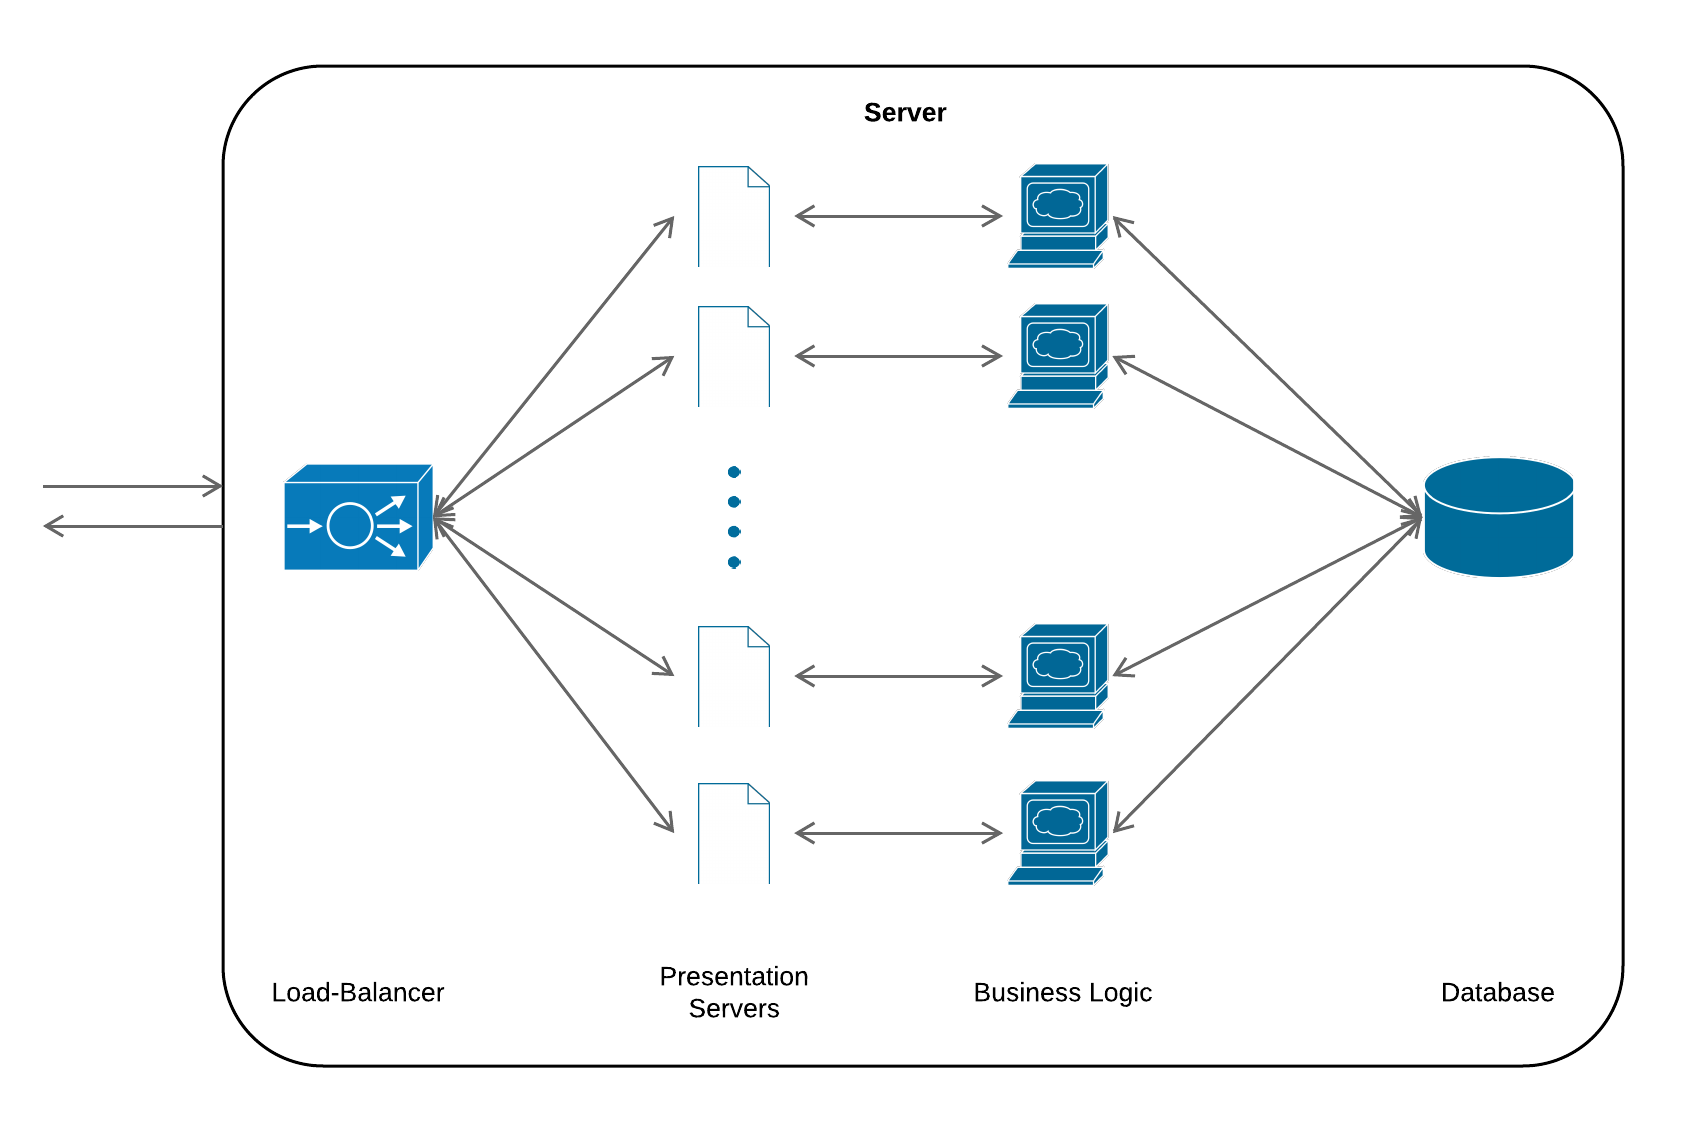
\includegraphics[scale=0.35]{Server}
	\caption{3-Tier Architectural}
	\label{server}
\end{figure}
In which, the server is divided into 3 part in addition to a database:
\begin{enumerate}
	\item \textbf{Load-Balancer}: The load-balancer will assign the coming request to a \textit{Presentation Server} to be further processed.
	\item \textbf{Presentation Server}: The Presentation Server is used to generate the file that requested by coming message.
	\item \textbf{Business Logic Device}: The Business Logic is used to gather and process the data that may used to generate the requested file.
\end{enumerate}
The general process when the server receive a request is:
\begin{enumerate}
	\item The Load-Balancer will first deliver the request to one of the Presentation Servers.
	\item The Presentation Server will ask Business Logic to provide the data that is required for generating file.
	\item The Business Logic will start to gather and process data, \textsl{e.g.} retrieve data from database. 
	\item The Business Logic provide the required data to Presentation Server.
	\item The Presentation Server generate the file by using these data and send it back to Load-Balancer.
	\item  The Load-Balancer send the file back to the client.
\end{enumerate}
Particularly, the database is not count as the part of 3-Tier Server Architectural.
\end{comment}
\end{document}